%
%  user2010_sna
%
%  Created by Drew Conway on 2010-06-15.
% 
%
\documentclass[xcolor=dvipsnames, 9pt]{beamer}

\newenvironment{code}{\begin{semiverbatim} \begin{footnotesize}}
{\end{footnotesize}\end{semiverbatim}}

\usepackage{graphicx}
\usepackage{amssymb}
\usepackage{amsfonts}
\usepackage{amsmath}
\usepackage{hyperref}
\usepackage{natbib}
\usepackage{color}
\usepackage{pdfsync}
\usepackage{chancery}
\usepackage{movie15}
\usepackage{pgfpages}
\usepackage{fancyvrb}
\usepackage{colortbl}
\usepackage{multirow}
\usepackage{ulem}

% \definecolor{white}{rgb}{255,255,255}
% \definecolor{darkred}{rgb}{0.5,0,0}
% \definecolor{darkgreen}{rgb}{0,0.5,0}
% \definecolor{lightblue}{rgb}{0,0,0.7}

% \hypersetup{colorlinks,
%   linkcolor=white,
%   filecolor=darkred,
%   urlcolor=lightblue,
%   citecolor=darkblue}

\usepackage{beamerthemesplit}
\usetheme{Copenhagen}
\usecolortheme[named=Violet]{structure} 
\setbeamertemplate{navigation symbols}{}
\setbeamertemplate{itemize items}[triangle]
\setbeamertemplate{enumerate items}[default]
%\setbeameroption{show notes on second screen}
%\logo{\includegraphics[width = 2cm]{nyulogo.png}}

\newcommand{\R}{\mathbb{R}}
\renewcommand{\d}{\mathsf{d}}
\newcommand{\dd}{\partial}
\newcommand{\E}{\mathsf{E}}
\newcommand{\bb}{\mathbf}

\title{Real-time network analysis in R using Twitter}
\author{Drew Conway}
\institute{New York University --- Department of Politics}
\date{July 22, 2010}

\begin{document} 

\begin{frame}[plain]
  \titlepage  
\end{frame}

\begin{frame}[plain]
    \frametitle{Standing on the shoulders of giants}
    Collection and parsing of Twitter data
    \begin{itemize}
        \item \texttt{twitteR}
        \item Jeff Gentry, Dept. of, Biostatistics --- Harvard University
    \end{itemize}
    \uncover<2->{Graph representations, analysis and visualization
    \begin{itemize}
        \item \texttt{igraph}
        \item G\'{a}bor Cs\'{a}rdi, Dept. of Biophysics --- Universit\'{e} de Lausanne (Switzerland)
    \end{itemize}}
    \uncover<3->{Data visualization
    \begin{itemize}
        \item ggplot2
        \item Hadley Wickham, Dept. of Statistics --- Rice University
    \end{itemize}}
\end{frame}


\section{Why use R to do SNA?} % (fold)
\label{sec:why_use_r_to_do_sna_}

\subsection{SNA Software Landscape} % (fold)
\label{sub:sna_software_landscape}

\begin{frame}[fragile]
    \frametitle{A bit on tools}
    The number of software suites and packages available for conducting social network analysis has exploded over the past ten years
    \begin{itemize}
        \item In general, this software can be categorized in two ways:
        \uncover<2->{\begin{itemize}
            \item \textbf{Type} - many SNA tools are developed to be standalone applications, while others are language specific packages 
            \item \textbf{Intent} - consumers and producer of SNA come from a wide range of technical expertise and/or need, therefore, there exist simple tools for data collection and basic analysis, as well as complex suites for advanced research
        \end{itemize}}
    \end{itemize}
    \vspace{1mm}
    \uncover<3->{\begin{tabular}{l | l | l }
        & \Large{\textit{Standalone Apps}} & \Large{\textit{Modules \& Packages}} \\ \hline
        \multirow{3}{*}{\Large{\textit{Basic}}} & - \href{http://www.casos.cs.cmu.edu/projects/ora/index.html}{ORA} (Windows) & - \href{http://www.libsna.org/}{libSNA} (Python) \\
        & - \href{http://www.i2.co.uk/products/analysts_notebook/}{Analyst Notebook} (Windows)  & - \href{http://www.southwindpress.com/urlnet/}{UrlNet} (Python)\\
        & - \href{http://www.andrew.cmu.edu/user/krack/krackplot.shtml}{KrakPlot} (Windows) & - \href{http://www.codeplex.com/NodeXL}{NodeXL} (MS Excel) \\ \hline
        \multirow{3}{*}{\Large{\textit{Advanced}}} & - \href{http://www.analytictech.com/ucinet6/ucinet.htm}{UCINet} (Windows) & - \href{http://networkx.lanl.gov/}{\color<5>{red}{NetworkX}} (Python) \\
        & - \href{http://vlado.fmf.uni-lj.si/pub/networks/pajek/}{Pajek} (Multi) & - \href{http://jung.sourceforge.net/}{JUNG} (Java) \\
        & - \href{http://nwb.slis.indiana.edu/}{\color<5>{red}{Network Workbench}} (Multi) & - \href{http://igraph.sourceforge.net/}{\color<5>{red}{igraph}} (Python, R \& Ruby) \\ \hline
    \end{tabular}}
    \uncover<4->{Many of the above tools have visualization components, but {several tools} are designed specifically for visualization: \href{http://www.graphviz.org/}{Graphviz}, \href{http://www.analytictech.com/downloadnd.htm}{NetDraw}, \href{http://www.tomsawyer.com/home/index.php}{Tom Sawyer}, \href{http://gephi.org/}{Gephi}, etc.} \uncover<5->{\alert{What I use}}
\end{frame}

% subsection sna_software_landscape (end)

\subsection{Pros and Cons of R} % (fold)
\label{sub:pros_and_cons_of_r}

\begin{frame}[fragile]
    \frametitle{Pros and Cons of SNA in R}
    \begin{columns}
        \column{0.5\textwidth}
        \underline{Pros}\\
        Diversity of tools available in R
            \begin{itemize}
                \small{\item Analysis - \tecxttt{\href{http://cran.r-project.org/web/packages/sna/index.html}{sna}}: sociometric data; \texttt{\href{http://hosho.ees.hokudai.ac.jp/~kubo/Rdoc/library/RBGL/html/00Index.html}{RBGL}}: Binding to Boost Graph Lib}
                \uncover<1->{\item Simulation - \texttt{\href{http://cran.r-project.org/web/packages/ergm/index.html}{ergm}}: exponential random graph; \texttt{\href{http://cran.r-project.org/web/packages/networksis/index.html}{networksis}}: bipartite networks}
                \item Specific use - \texttt{\href{http://cran.r-project.org/web/packages/degreenet/index.html}{degreenet}}: degree distribution; \texttt{\href{http://toreopsahl.com/}{tnet}}: weighted networks
            \end{itemize}
        \uncover<2->{Built-in visualization tools
        \begin{itemize}
            \small{\item Take advantage of R's built-in graphics tools}
        \end{itemize}
        \begin{tabular}{c c c}
            \href{http://igraph.sourceforge.net/images/screenshots/tkplot.png}{\includegraphics[width=1.3cm]{../images/tkplot.png}}&\href{http://igraph.sourceforge.net/images/screenshots/fastgreedy.png}{\includegraphics[width=1.3cm]{../images/fastgreedy.png}}&\href{http://igraph.sourceforge.net/images/screenshots/mst.png}{\includegraphics[width=1.3cm]{../images/mst.png}}
        \end{tabular}} \\
        \uncover<3->{Immediate access to more stats
        \begin{itemize}
            \item \scriptsize{Perform SNA and network based econometrics ``under the same roof"}
        \end{itemize}}
        \column{0.5\textwidth}
        \underline{Cons} \\
        \uncover<4->{\small{Steep learning curve for SNA novices}
            \begin{itemize}
                \item \small{As with most things in R, the network analysis packages were designed by analysts for analysts
                \item These tools require at least a moderate familiarity with network structures and basic metrics}}
                \uncover<5->{\tiny{\begin{block}{Structural Holes}}
                       \tiny{Burt's constraint is higher if ego has less, or mutually stronger related (i.e. more redundant) contacts. Burt's measure of constraint, C[i], of vertex i's ego network V[i]}
                    \end{block}}
            \end{itemize}
        \uncover<6->{\small{In ability to exchange data between other network analysis packages}
        \begin{itemize}
            \scriptsize{\item \small{\texttt{statnet} library powerful for modeling}
            \item \texttt{igraph} and \texttt{statnet} represent networks in different ways
            \item Difficult to exchange data between libraries}
        \end{itemize}}
        \vspace{2mm}
        \end{columns}
\end{frame}

% subsection pros_and_cons_of_r (end)

\section{Examples of SNA in R} % (fold)
\label{sec:examples_of_sna_in_r}

\subsection{Basic SNA} % (fold)
\label{sub:basic_sna}

\begin{frame}[fragile]
    \frametitle{Comparing two network metrics to find key actors}
    Often social network analysis is used to identify key actors within a social group.  To identify these actors, various centrality metrics can be computed based on a network's structure
    \begin{itemize}
        \item Degree (number of connections)
        \item Betweenness (number of shortest paths an actor is on)
        \item Closeness (relative distance to all other actors)
        \item Eigenvector centrality (leading eigenvector of sociomatrix)
    \end{itemize}
    \uncover<2->{One method for using these metrics to identify key actors is to plot actors' scores for Eigenvector centrality versus Betweenness.  Theoretically, these metrics should be approximately linear; therefore, any non-linear outliers will be of note.
    \begin{itemize}
        \item An actor with very high betweenness but low EC may be a critical gatekeeper to a central actor
        \item Likewise, an actor with low betweenness but high EC may have unique access to central actors
    \end{itemize} }
\end{frame}

\begin{frame}[fragile]
    \frametitle{Finding Key Actors with R}
    For this example, we will use the main component of the social network collected on drug users in Hartford, CT.\footnote{Weeks, et al (2002) \url{http://dx.doi.org/10.1023/A:1015457400897}}  The network has 194 nodes and 273 edges.
    \uncover<2->{\begin{block}{Load the data into igraph}}
        \begin{code}
\uncover<2->{library(igraph)
G<-read.graph("drug_main.txt",format="edgelist")
G<-as.undirected(G)
\alert{# By default, igraph inputs edgelist data as a directed graph.}
\alert{# In this step, we undo this and assume that all relationships are reciprocal.}}
        \end{code}
    \end{block}
    \uncover<3->{\begin{block}{Store metrics in new data frame}}
        \begin{code}
\uncover<3->{cent<-data.frame(bet=betweenness(G),eig=evcent(G)\$vector)
\alert{# evcent returns lots of data associated with the EC, but we only need the 
# leading eigenvector}
res<-lm(eig~bet,data=cent)\$residuals
cent<-transform(cent,res=res)
\alert{# We will use the residuals in the next step}}
        \end{code}
    \end{block}
\end{frame}

\begin{frame}[fragile]
    \frametitle{Finding Key Actors with R}
    \begin{columns}
        \column{0.4\textwidth}
            \small{\begin{block}{Plot the data}}
                \begin{code}
\scriptsize{library(ggplot2)
\alert{# We use ggplot2 to make things a 
# bit prettier}
p<-ggplot(cent,aes(x=bet,y=eig,
    label=rownames(cent),colour=res,
    size=abs(res)))+xlab("Betweenness 
    Centrality")+ylab("Eigenvector 
    Centrality")
\alert{# We use the residuals to color and
# shape the points of our plot,
# making it easier to spot outliers.}
p+geom_text()+opts(title="Key Actor 
    Analysis for Hartford Drug Users")
\alert{# We use the geom_text function to plot 
# the actors' ID's rather than points
# so we know who is who}}
                \end{code}
            \end{block}
        \column{0.6\textwidth}
            \uncover<2->{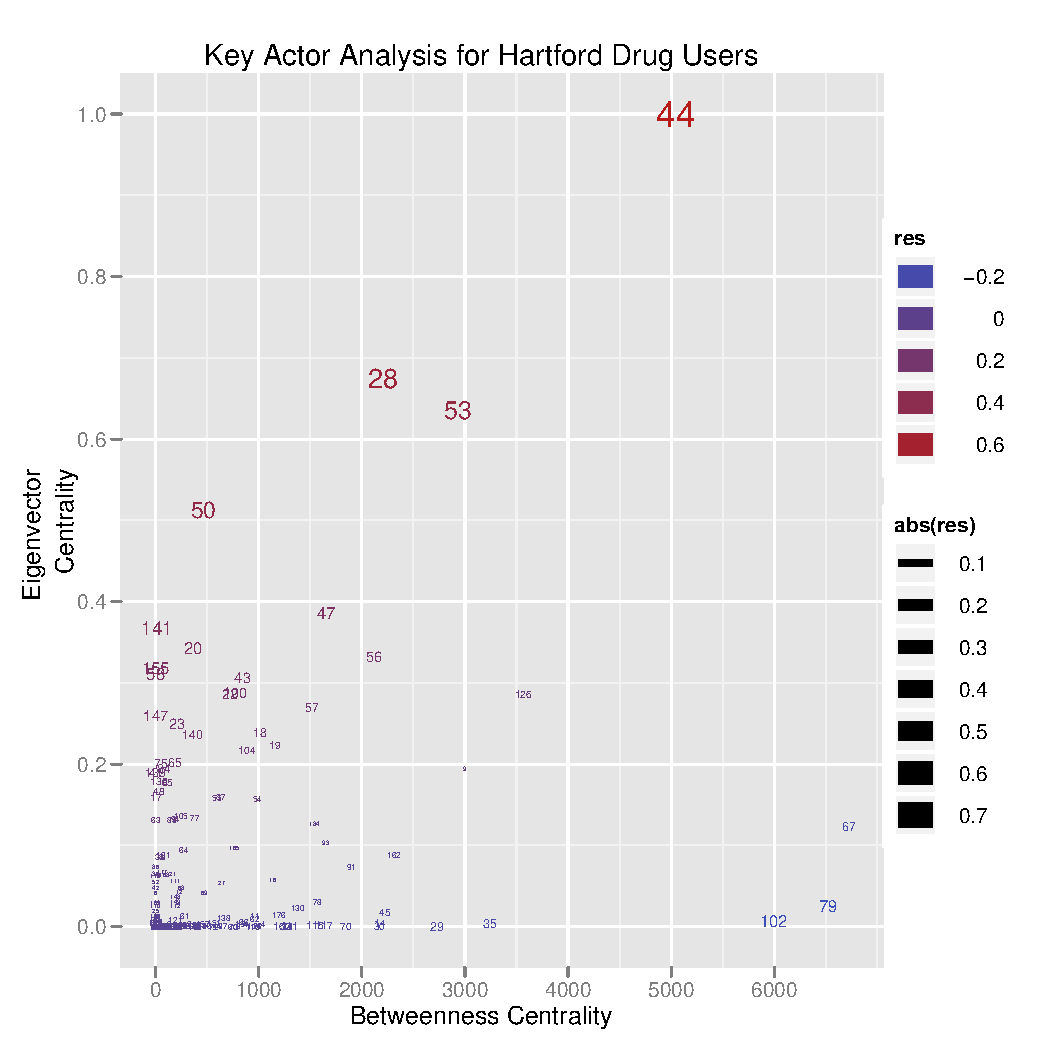
\includegraphics[width=70mm]{../images/key_actor_analysis.pdf}}
    \end{columns}
\end{frame}

\section{Digging into data} % (fold)
\label{sec:digging_into_data}

\subsection{Getting data} % (fold)
\label{sub:where_to_get_data}

\begin{frame}[fragile]
    \frametitle{Where to get social graph data}
    Recently, there has been an explosion of resources for scraping social graph
    \begin{table}
        \centering
        \scriptsize{
        \begin{tabular*}{.99\textwidth}{c|l|l}
        Service & Data & API Docs \\ \hline \hline
        \includegraphics[height=4mm]{../images/twitter_logo.png} & Following(ers), @-replies, date/time/geo & \url{http://apiwiki.twitter.com/} \\ \hline
        \includegraphics[height=4mm]{../images/facebook_logo.jpg} & Friends, Wall Posts, date/time & \url{http://developers.facebook.com/docs/api} \\ \hline
        \includegraphics[height=4mm]{../images/Newgooglelogo.png} & All SocialGraph relationships & \url{http://code.google.com/apis/socialgraph/} \\ \hline
        \includegraphics[height=4mm]{../images/foursquare.png} & Friends, Check-ins & \url{http://foursquare.com/developers/} \\ \hline
        \includegraphics[height=3mm]{../images/Hunch_com_logo.png} & ``Taste graph", recommendations  & \url{http://hunch.com/developers/} \\ \hline
        \includegraphics[height=4mm]{../images/nytlogo.png} & Congressional votes, campaign finance & \url{http://developer.nytimes.com/docs}
        \end{tabular*}}
    \end{table}
    \uncover<2->{There is clearly no shortage of data
    \begin{itemize}
        \item Each service provides different relational context
        \item Data formats are generally JSON, Atom, XML, or some combination
        \item For a more extensive list of API resources, see HackNY wiki of \href{http://hackny.org/wiki/index.php?title=Main_Page#Start_ups_websites}{local startups}
    \end{itemize}}
\end{frame}

\begin{frame}[fragile]
    \frametitle{Why use Twitter for analyzing networks?}
    \begin{columns}
        \column{.6\textwidth}
        Unprecedented scale and accessibility
           \begin{itemize}
               \item Twitter provides free and open (rate-limited) access to their data
               \item The amount of data pushed to daily is enormous
               \item ``Following'' structure natural social network
           \end{itemize}
        \column{.4\textwidth}
            \uncover<2->{\includegraphics[width=4.5cm]{../images/chart-tweets-per-day3.png}}
    \end{columns}
    \uncover<3->{Rich meta-data
    \begin{itemize}
        \item Context of relationships can be inferred by Tweet content
        \item All relationships longitudinal
        \item Many Tweets contain geospatial data
    \end{itemize}}
    \uncover<4->{Easy integration into R
    \begin{itemize}
        \item Data easily parsed with \href{http://cran.r-project.org/web/packages/twitteR/}{\texttt{twitteR}} library (\href{http://twitter.com/geoffjentry}{@geoffjentry})
        \item Quickly build edgelist structures
        \item Can use libraries such as \href{http://crantastic.org/packages/tm}{\texttt{tm}} and \texttt{ts} for text and longitudinal analysis
    \end{itemize}}
\end{frame}

\begin{frame}[fragile]
    \frametitle{Infochimps.org}
    \begin{columns}
        \column{.5\textwidth}
            \includegraphics[width=5.5cm]{../images/home_450.png}
        \column{.5\textwidth}
        In addition to pulling the data yourself, Infochimps.org also offers large data sets for download (for a fee)
        \begin{itemize}
            \item Monthly Twitter census data
        \end{itemize}
        Infochimps also has a set of internally defined Twitter metrics that can be accessed freely via an API (\url{http://api.infochimps.com/})
        \begin{itemize}
            \item \texttt{trstrank} --- a version of Google's PageRank for Twitter
            \item Influence metrics --- Twitter user ``retweets'' and @ replies
        \end{itemize}
    \end{columns}
\end{frame}


\subsection{Getting data out of Twitter into R} % (fold)
\label{sub:getting_data_out_of_twitter_into_r}

% subsection getting_data_out_of_twitter_into_r (end)

\begin{frame}[fragile]
    \frametitle{Getting started}
    \begin{block}{Load libraries and initialize Twitter session}
\begin{code}
\alert<2>{# We will use ggplot2 for later visualization
library(twitteR)
library(igraph)
library(ggplot2)}

\alert<3>{# Initialize a session to gather dat
user<-"your.name"
pass<-"your.pass"
twit<-initSession(user,pass)}

\alert<4>{# Get all the users from the last 100 tweets containing some hashtag
hashtag<-"my.hashtag"
hash.tweets<-get.hashtag(hashtag)
hash.users<-users.from.statuses(hash.tweets)}
\end{code}
    \end{block}
\end{frame}

\begin{frame}[fragile]
    \frametitle{Create several helper functions to generate network data from Twitter}
    \begin{block}{}
    \begin{code}
\tiny{\alert<2>{# Function for converting twitteR object data to vector
friend.vector<-function(friends) \{
    v<-c()
    for(i in 1:length(friends)) \{v<-append(v,as.character(screenName(friends[[i]])))\}
    return(v)\}}
\alert<3>{# Function for generating edgelists
create.adj<-function(seed) \{
    u<-getUser(seed)
    # Cannot create network data from protected accts
    if(protected(u)==FALSE) \{
        outdegree<-userFriends(u,twit)
        friends<-friend.vector(outdegree)
        return(list(adj.list=cbind(seed,friends),seed.friends=friends))
    \}
    else \{
        return(list(adj.list=NA,seed.friends=NA))
    \}\}}
\alert<4>{# Get the last 100 tweets containing the given hashtag
get.hashtag<-function(hashtag,session=getCurlHandle()) \{
    search.url<-paste("http://search.twitter.com/search.json?q=%23",hashtag,"&rpp=100",sep="")
    out <- getURL(search.url, curl = session)
    jsonList <- twFromJSON(out)[[1]]
    return(sapply(jsonList, buildStatus))\}}
\alert<5>{# Get the users from a list of tweets
users.from.statuses<-function(status.list) \{
    users<-c()
    for(i in 1:length(status.list)) \{
        users<-append(users,(screenName(status.list[[i]])))
    \}
    return(unique(users))\}}}
\end{code}
    \end{block}
\end{frame}

\begin{frame}[fragile]
    \frametitle{Build the network}
    \begin{block}{}
        \begin{code}
\alert<2>{# We now build the network, but we have to make sure the initial seed is not protected
seed.user<-1
while(protected(getUser(hash.users[seed.user]))) \{seed.user<-seed.user+1\}}
\alert<3>{# Now create the edgelists for all uses 
for(u in seed.user:length(hash.users)) \{
    if(u==seed.user) \{
        hash.list<-create.adj(hash.users[u])
        hash.el<-hash.list\$adj.list
    \}}
    \alert<4>{else \{
        current.list<-create.adj(hash.users[u])
        current.el<-current.list\$adj.list
        if(is.na(current.el)) \{
            print(paste(hash.users[u]), ``has a protected account--ignoring'')
        \}}
        \alert<5>{else \{
            hash.el<-rbind(hash.el,current.el)
        \}
    \}
\}}
        \end{code}
    \end{block}
\end{frame}


\section{Live demonstration} % (fold)
\label{sec:live_demonstration}

\begin{frame}[fragile]
    \frametitle{Live demo}
    \begin{center}
        \Huge{\sout{Live}Pre-loaded demonstration time!\\ \#user2010}\\
        \vspace{2cm}{\large{All code available at \url{http://www.drewconway.com/zia}}}
    \end{center}
\end{frame}

% section live_demonstration (end)




\end{document}
